% Use only LaTeX2e, calling the article.cls class and 12-point type.

\documentclass[11pt]{article}
\usepackage[round,semicolon]{natbib}
\usepackage[margin=1.3in]{geometry}
\usepackage{kpfonts}

\usepackage{seqsplit}

\usepackage{newfloat}
\usepackage[labelfont=bf]{caption}
\usepackage{nameref}
\usepackage{rotating}
\usepackage{color}
\usepackage{float}

\setcounter{topnumber}{8}
\setcounter{bottomnumber}{8}
\setcounter{totalnumber}{8}

\usepackage{newfloat}
\DeclareFloatingEnvironment[name={Supplementary Figure}]{suppfigure}

\definecolor{darkblue}{rgb}{0, 0.0, 0.6}

\usepackage{hyperref}
\hypersetup{colorlinks,citecolor=blue,linkcolor=darkblue,urlcolor=blue}

\usepackage{seqsplit}

\usepackage{array}
\newcolumntype{R}[1]{>{\raggedright\arraybackslash}p{#1}}
\newcolumntype{C}[1]{>{\centering\let\newline\\\arraybackslash\hspace{0pt}}m{#1}}

\newcommand{\comment}[1]{{\color{red}(\textsl{#1})}}

\usepackage{setspace}

\renewcommand{\topfraction}{1}
\renewcommand{\bottomfraction}{1}
\renewcommand{\textfraction}{0}
\renewcommand{\floatpagefraction}{1}

%\renewcommand{\abstractname}{\large SUMMARY}


\title{Contrasting the potential for viral escape from broad and narrow antibodies by complete mapping of the antigenic effects of single amino-acid mutations to influenza hemagglutinin}

\author
{Michael B. Doud$^{1,2,3,\dagger}$, Juhye M. Lee$^{1,2,3,\dagger}$, and Jesse D. Bloom$^{1,2,*}$\\
\\
\scriptsize{$^1$Basic Sciences and Computational Biology Program, Fred Hutchinson Cancer Research Center}\\
\scriptsize{$^2$Department of Genome Sciences and $^3$Medical Scientist Training Program, University of Washington} \\
\scriptsize{Seattle, WA, USA} \\
\scriptsize{$^{\dagger}$These authors contributed equally} \\
\scriptsize{$^*$Correspondence: \href{jbloom@fredhutch.org}{jbloom@fredhutch.org}}
}

\date{}


\begin{document}

\maketitle
\onehalfspacing

\begin{abstract}
Broadly neutralizing antibodies are of great interest as therapeutics to treat influenza and are the desired products of future universal influenza vaccines. 
It is important to understand viral potential for escape from antibodies and to develop ways to compare how easy or difficult it is for viral escape between various antibodies. 
We previously demonstrated a method to measure the effects of all amino-acid mutations in influenza HA on viral escape from neutralizing antibodies. 
Here we apply this technique to 'broadly neutralizing' antibodies with reactivity spanning multiple influenza subtypes, including antibodies targeting the HA receptor-binding site and stalk domain. We find quantitatively similar distributions of escape mutations to a relatively broad antibody targeting the receptor-binding site (s139) and to several narrow-specificity antibodies targeting nearby antigenic regions of the head domain (H17-L19, others?). 
In contrast to the ease of escape from head-binding antibodies of various breadths, stalk-binding antibodies can only be evaded by a paucity of mutations with relatively small effects.  
For the antibodies studied here, antibody breadth is not an indicator of difficulty for viral escape.  
Instead, targeting a mutationally intolerant epitope in the stalk region seems to limit viral escape mutations to a few relatively ineffective options
\end{abstract}

\section*{INTRODUCTION}
Broadly neutralizing antibodies against influenza virus are of great interest... \cite{corti2017tackling}. 

% blurbs about the specific antibodies we use here:
C179 isolation and escape mutant selection \cite{okuno1993common}.
C179 structure with 1957 H2, binding data to many strains, and citations to older studies demonstrating C179 cross-neutralization to H1, H2, H5, H6, and H9:  \cite{dreyfus2013structure}.
FI6v3 was isolated... \cite{corti2011neutralizing}.
S139/1 isolation and selection of escape mutants from Aichi H3, Adachi H2, and WSN H1: \cite{yoshida2009cross}.
S139/1 structure with Victoria75 H3 and binding/neutralization data: \cite{lee2012heterosubtypic}.

Recently we have described new technologies... \cite{doud2017complete, dingens2017comprehensive}.


\section*{RESULTS}

\subsection*{First subsection.}
Some text

\begin{figure}
\centerline{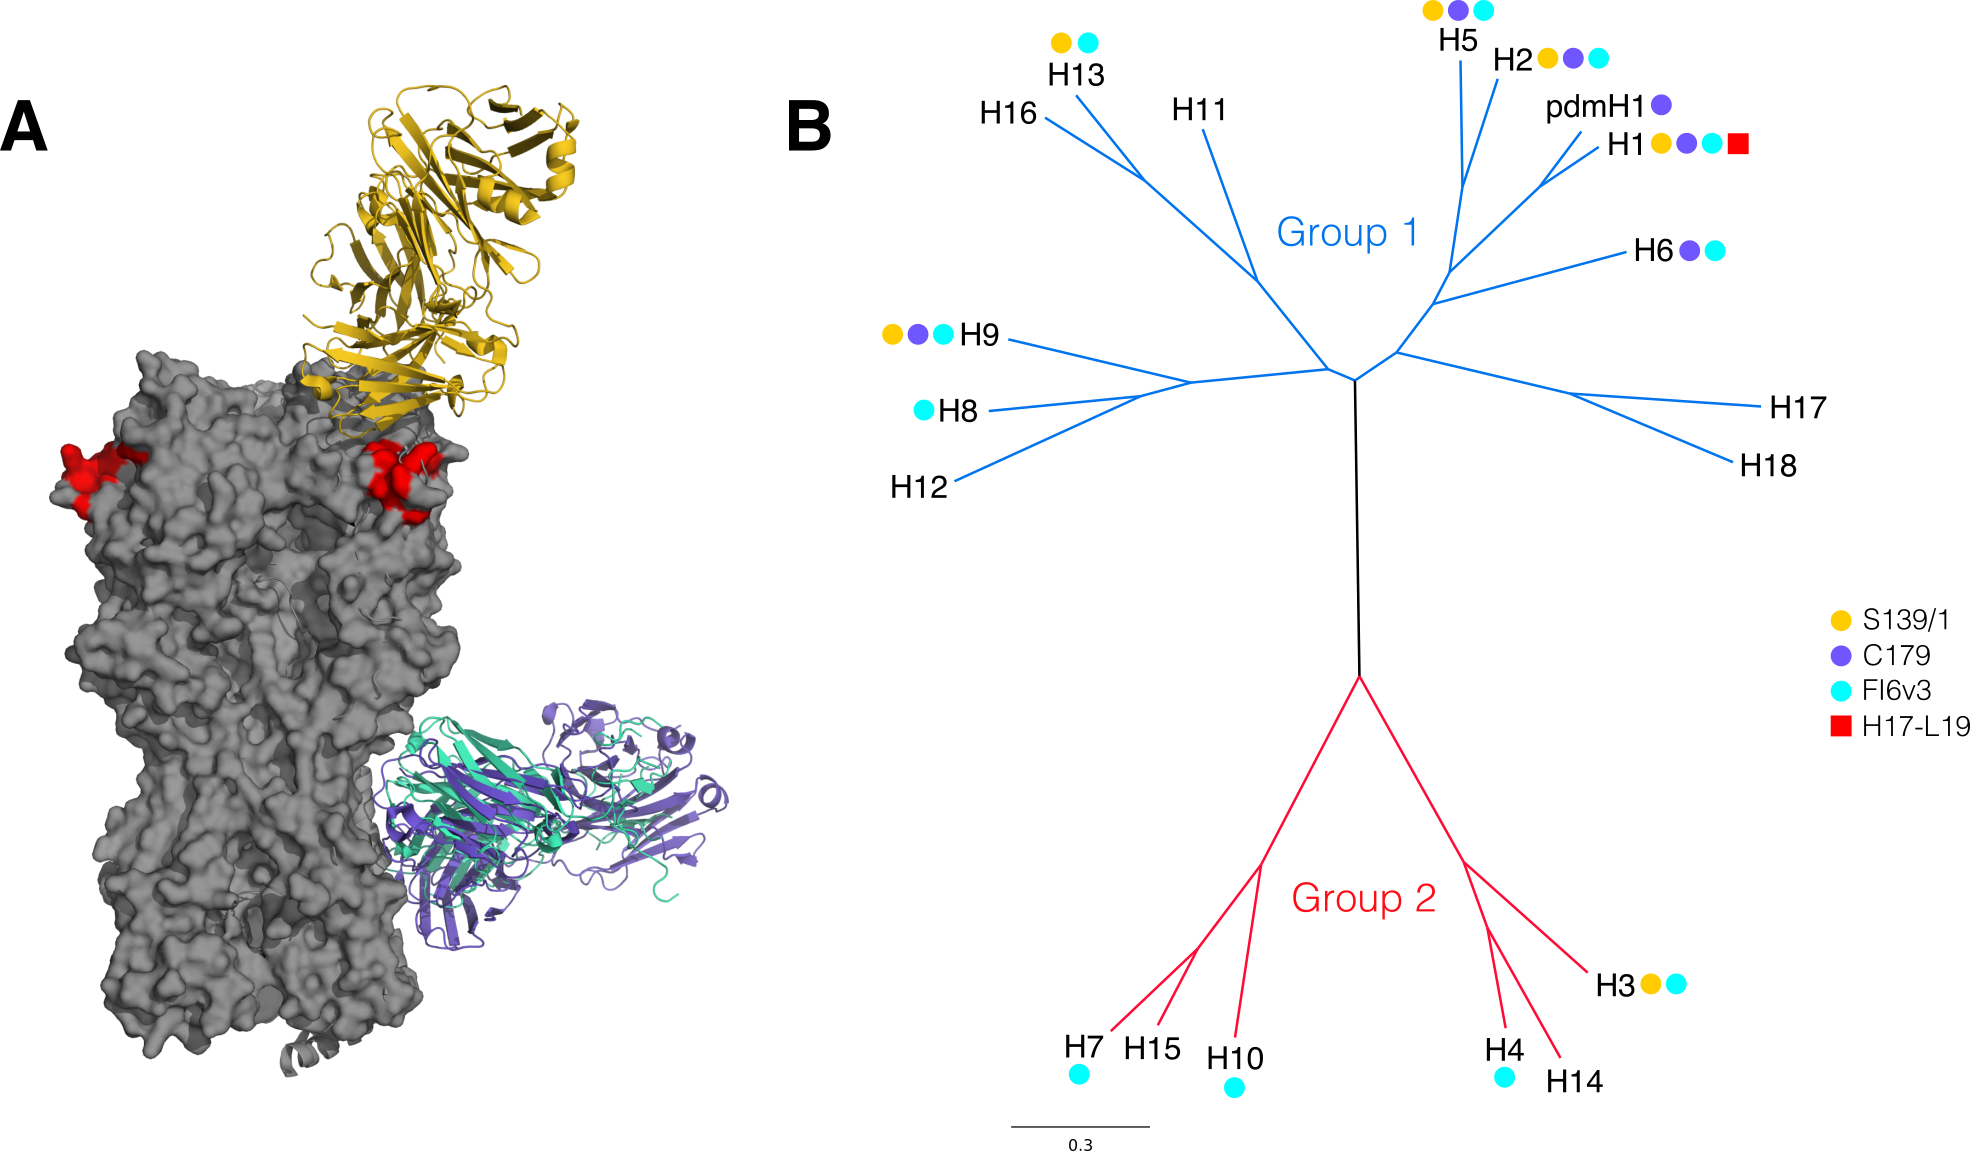
\includegraphics[width=\textwidth]{figs/antibody_summary_fig/fig.png}}
\caption{\label{fig:antibody_summary}
CAPTION}
\end{figure}

\section*{DISCUSSION}
Some discussion

\clearpage

\section*{METHODS}
\subsection*{Antibodies}
FI6v3 was expressed and purified by the Fred Hutchinson Cancer Research Center protein expression core \comment{i think?}.
C179 was purchased from Takara Bio Inc (Catalog \# M145).
S139/1 heavy and light chain variable sequences were obtained from PDB ID 4GMS~\cite{lee2012heterosubtypic} and expressed and purified by the Fred Hutchinson Cancer Research Center protein expression core.

\subsection*{Mutant virus selections with antibody}
Library selections, deep sequencing, and computation of mutation differential selection were performed as previously described~\cite{doud2017complete}. Briefly, ...

\subsection*{Computation of the fraction $\phi_{r,a}$ of each mutation that escapes antibody neutralization}
\comment{depending on how much of paper focus is on this new metric, some of this rationale might be better placed in the results section}

Mutation differential selection values $s_{r,a}$ reflect the enrichment of a mutation in an antibody-selected sample relative to a mock-selected control. 
The extent of these mutation enrichments are dependent on the stringency of the neutralization: as the concentration of an antibody used to neutralize the mutant virus library is increased, a larger proportion of the virus library is neutralized, and escape mutants become more enriched in the antibody-selected sample relative to the control sample~\cite{doud2017complete}.
Consequently, due to differences in the concentrations and potencies of various antibodies used in mutational antigenic profiling, quantitative comparisons of the effects of mutations on neutralization escape between various antibodies is confounded by differences in neutralization stringency across experiments.

We defined a new metric that accounts for the neutralization stringency of each experiment so that quantitative comparisons can be made between experiments with varying neutralization stringencies.
This new measure, $\phi_{r,a}$, is roughly analogous to the fraction of mutant viruses carrying mutation $a$ at site $r$ that escape neutralization by a given antibody.
The computation of $\phi_{r,a}$ incorporates information about the stringency of neutralization. 
We define this as  $\gamma$ = (100 - \% neutralization)/100), the fraction of library remaining infectious after antibody neutralization measured by qRT-PCR for each antibody-selection experiment as previously described~\cite{doud2017complete}.

Define $\hat{n}_{r,a}^{sel}$ and $\hat{n}_{r,a}^{mock}$ as the number of error-corrected counts of amino-acid mutant $a$ at site $r$ as defined in~\cite{doud2017complete}, and $N_r^{sel}$ and $N_r^{mock}$ be the total counts at site $r$, as specified for either an antibody selection or matched mock condition.
Let $P$ be a pseudocount (default to 5 in these analyses) added to amino-acid counts, and let $f_{r}^{sel}$ and $f_{r}^{mock}$ be relative depths of the selected and mock samples at site $r$ for the purposes of scaling the pseudocount by relative read depth as previously described~\cite{doud2017complete}.

Define the pseudocount-adjusted frequency $\rho$ of mutant $a$ at site $r$ in selected and mock samples to be:
$$\rho_{r,a}^{sel} = \frac{n_{r,a}^{sel}+f_r^{sel}\times P}{N_r^{sel}+f_r^{sel}\times  P}$$
$$\rho_{r,a}^{mock} = \frac{n_{r,a}^{mock}+f_r^{mock}\times P}{N_r^{mock}+f_r^{mock}\times  P}$$

We define $\phi_{r,a}$ as the net `fraction' of mutant $a$ at site $r$ escaping neutralization (above the average escape fraction $\gamma$), and compute this as:
$$\phi_{r,a} = \frac{\gamma \times \rho_{r,a}^{sel}}{\rho_{r,a}^{mock}} - \gamma$$

By this definition, mutations with no effect on antibody escape will have $\phi_{r,a} =0$, and mutations completely escaping antibody will have $\phi_{r,a} \approx 1$.
Care should be taken in interpreting the absolute values of $\phi$, however, since the choice of pseudocount affects the range of $\phi$ values (but not, importantly, the relationships of $\phi$ distributions across antibodies).
We have found that a value of $P=5$ pseudocounts results in $\phi$ values that are roughly bounded from 0 to 1, and consistently use $P=5$ all analyses.

\subsection*{Data availability and source code}
Deep sequencing data has been deposited at the Sequence Read Archive under BioSample accession (\comment{should probably deposit all the new data into the existing biosample SAMN05789126 (Sample name: WSN/1933 HA mutant libraries selected by monoclonal antibodies), which is under bioproject PRJNA309339}).




\clearpage

\small
\subsection*{ACKNOWLEDGMENTS}
This work was supported by grants R01GM102198 and R01AI127893 from the NIGMS and NIAID of the NIH.
MBD was supported in part by training grant T32AI083203 from the NIAID of the NIH.
JML was supported in part by \comment{CIDID grant}.
The research of JDB is supported in part by a Faculty Scholar Grant from the Howard Hughes Medical Institute and the Simons Foundation.

\bibliographystyle{mbe}
\bibliography{references.bib}

\clearpage
\normalsize

\section*{Supplementary Material}


\end{document}
